\section{Analyse d'évaluation originale}

\textbf{\color{red}Note : Le document original fait 13 pages. Je pense qu'il serait plus intéressant de la tronquer pour garder les parties en lien avec la différenciation et déposer le document original tel que rendu à ma tutrice dans l'espace de téléchargement du site web.}

\subsection{Contexte de l'évaluation}
%La présentation de cette évaluation :la classe, le(s) titre(s) de la (des) séquence(s) concernée(s) par cette  évaluation, le type d'évaluation  présentée  (diagnostique,  formative,  sommative),  sa  place  par  rapport  à  la ou les séquence(s), le déroulement prévu (durée, mise en œuvre), les outils disponibles pour les élèves

L'évaluation a été donnée aux élèves de la classe 5\up{e} \textsc{Monet}. Elle portait sur les séquences \textit{Symétrie axiale et symétrie centrale} (débutée le 1\up{er} octobre) et \textit{Nombres relatifs} (débutée le 12 novembre). C'était la deuxième évaluation sommative portant sur la symétrie centrale et la première portant sur les nombres relatifs. 

\subsubsection*{Place de l'évaluation dans la séquence de géométrie}
La première évaluation sommative était un devoir à la maison où les élèves devaient compléter le dessin d'un papillon à l'aide de la symétrie axiale et de la symétrie centrale (rendu le 23 octobre, figure disponible dans l'annexe \ref{papillon}). Cette évaluation-ci a été donnée à la fin de la séquence, clôturée dix jours plus tôt.

\subsubsection*{Place de l'évaluation dans la séquence des nombres relatifs}
Cette évaluation a été donnée en milieu de séquence. Cela a eu des conséquences sur le contenu donné aux élèves (voir partie \ref{prep}).

\subsubsection*{Déroulement et outils}\label{cocottes}

L'évaluation était prévue pour durer une séance (soit 57 minutes). Les élèves avaient eu pour consigne d'apporter leur matériel de géométrie (règle, équerre, compas, rapporteur) et des fiches méthodologiques préparées en amont. Le texte des fiches méthodologiques est disponible dans l'annexe \ref{methodo}.\\

Les élèves qui le souhaitaient avaient la possibilité de me demander des cocottes en papier fabriquées par leurs soins et stockées dans une de mes salles de classe pour les aider à visualiser la symétrie axiale et la symétrie centrale.\\

Je suis régulièrement intervenue auprès de certains élèves pour leur apporter un soutien (l'un des élèves est en attente d'un AVS et se décourage en évaluation, deux autres se découragent très vite et un dernier est allophone et a parfois besoin de consignes reformulées). J'avais également apporté quelques outils de géométrie supplémentaires venant de la salle d'un de mes collègues pour pallier les oublis des élèves.

\newpage
\subsection{Préparation et déroulement de l'évaluation}
\subsubsection*{Objectifs de l'évaluation}\label{prep}
%b)les  objectifs  visés  (connaissances,  capacités  et  compétences),  les  choix  de  contenus effectués
Lors de cette évaluation, les objectifs ciblés étaient les suivants :
\begin{itemize}
    \item construire une figure géométrique avec soin et précision ;
    \item savoir coder une figure et laisser apparents les traits de construction ;
    \item savoir différencier la symétrie axiale et la symétrie centrale ;
    \item restitution de connaissances sur la construction et le repérage sur un axe gradué,
    \item doublée d'une évaluation de leur capacité à communiquer ;
    \item savoir additionner des nombres relatifs ;
    \item rédiger avec soin.
\end{itemize}

Me concernant, cela me permettait de faire une nouvelle évaluation diagnostique à partir de l'exercice 1 pour voir la progression des élèves (exercice très proche de ce qui leur avait été demandé lors du devoir à la maison) et de vérifier que je pouvais passer à la suite de ma séquence sur les nombres relatifs (repérage dans un repère cartésien).\\

Mes évaluations d'une heure contiennent autant que possible un exercice axé sur la communication en français. Ici, elle est évaluée à l'aide de l'exercice 3.\\

L'exercice 2 leur permettait de mettre en application les propriétés de conservation de la symétrie centrale s'ils le souhaitaient, avec la possibilité d'utiliser une autre stratégie s'ils avaient besoin de plus de temps pour s'approprier cette partie de la séquence. ces propriétés devaient être très prochainement réinvesties dans la séquence de géométrie suivante, ce n'était donc pas un problème que les élèves n'utilisent pas tous cette stratégie.\\

Les exercices 3 et 4 sont très proches d'exercices d'applications à cause de sa place dans la séquence. À ce sujet, j'ai supprimé une adaptation de l'\href{http://cache.media.education.gouv.fr/file/Nombres_relatifs/03/5/RA16_C4_MATH_nombres_relatifs_labyrinthe_N.D_552035.pdf}{exercice du labyrinthe} 
(\url{http://cache.media.education.gouv.fr/file/Nombres_relatifs/03/5/RA16_C4_MATH_nombres_relatifs_labyrinthe_N.D_552035.pdf}) initialement prévu, suite à une première application en classe qui s'est révélée négative, les élèves ayant eu des difficultés à comprendre l'énoncé.

\subsection{Analyse a priori}
%c)les  difficultés  prévisibles  des  élèves,  les  indicateurs  de  réussite  prévus  (en  lien  avec  le barème  et  es  compétences  ciblées),  éventuellement  des  éléments  de  différenciation envisagés
À ce stade de l'année, certains élèves avaient besoin de recourir aux cocottes en papier pour visualiser les effets de la symétrie axiale et de la symétrie centrale (voir partie \ref{cocottes}). D'autres commençaient à se contenter d'utiliser simplement leurs mains. Les deux exercices de la partie géométrie portaient volontairement chacun sur la symétrie axiale ou la symétrie centrale pour estimer le nombre d'élèves qui substitueraient la symétrie centrale par la symétrie axiale.\\

Lors de la création de l'exercice 2, j'ai pensé à ajouter la question à droite demandant aux élèves de cocher la stratégie qu'ils avaient employée. Cela ne faisait pas partie de mes objectifs initiaux, mais je voulais estimer le nombre d'élèves qui avaient suffisamment de recul pour déterminer la stratégie qu'ils utilisaient. Il y a eu quelques erreurs et un certain nombre d'élèves n'a pas répondu à cette question. Cela participe des éléments de différenciation prévus lors de cette évaluation.\\

Les indicateurs de réussite sont disponibles dans l'annexe \ref{comp}. Sur conseil de ma tutrice terrain, Mme \textsc{Hizembert}, j'ai voulu proposer une évaluation par compétences en plus de la notation chiffrée en cours dans mon établissement.\\

Un autre élément de différenciation portait sur le nombre d'erreurs que les élèves détecteraient dans l'exercice 3. En particulier, je m'attendais à voir "deux graduations sont suffisantes" peu citée en raison du fait que j'avais peu insisté dessus en classe. Je m'attendais également à voir quelques erreurs dans la manière de poser le calcul dans l'exercice 4 en raison du fait que la notion était encore assez nouvelle, malgré l'attention portée à préparer particulièrement cette partie de l'évaluation.

\subsection{Préparation en amont}
%d)l'aide à la préparation de cette évaluation par les élèves éventuellement mise en place 
Les jours précédent cette évaluation, j'ai axé mes questions flash sur des exercices de calcul mental ou des calculs facilités par une représentation graphique avec les axes pour bien travailler les sommes de nombres relatifs. J'ai également demandé à des élèves de faire des restitutions de connaissances orales.
Pour la partie géométrie, nous avons travaillé ensemble à l'élaboration des textes fiches de méthodologie présentes dans l'annexe \ref{methodo}. Les élèves avaient l'autorisation de les reproduire sur des feuilles cartonnées et de les apporter lors de l'évaluation.

\subsection{Écart entre l'analyse a priori et le déroulement réel}
%e)le  déroulement  réel  et  l'analyse  des  différences  entre  le  déroulement  prévu  et  le déroulement réel (durée, demandes d'aides, etc.) 
Premier constat : peu d'élèves avaient créé et apporté leurs fiches de méthodologie. La raison évoquée plus tard était qu'ils avaient le sentiment de tricher. C'était la première fois qu'ils utilisaient ce type de matériel.\\

Second constat : une proportion d'élèves plus importante que je le pensais s'est passée de l'utilisation des cocottes.\\

Globalement, l'évaluation s'est déroulée comme je le pensais. Une élève en particulier avait bien assimilé que j'attendais d'eux du soin et de la précision et a perdu ses moyens quand elle s'est rendue compte que sa feuille avait été abîmée par son compas. Le manque de support sous sa feuille en était la cause.

\newpage
\subsection{Productions d'élèves}
%f)l'analyse  de  deux  production(s)  d'élève(s)  (copies  ou  extraits  de  copies,  corrigés  et annotés), à joindre en annexe 

J'ai choisi de me focaliser sur l'exercice 2 de l'évaluation, reproduit ci-dessous. Certaines réponses m'avaient interpelée lors de la correction.
\begin{figure}[!h]
    \center{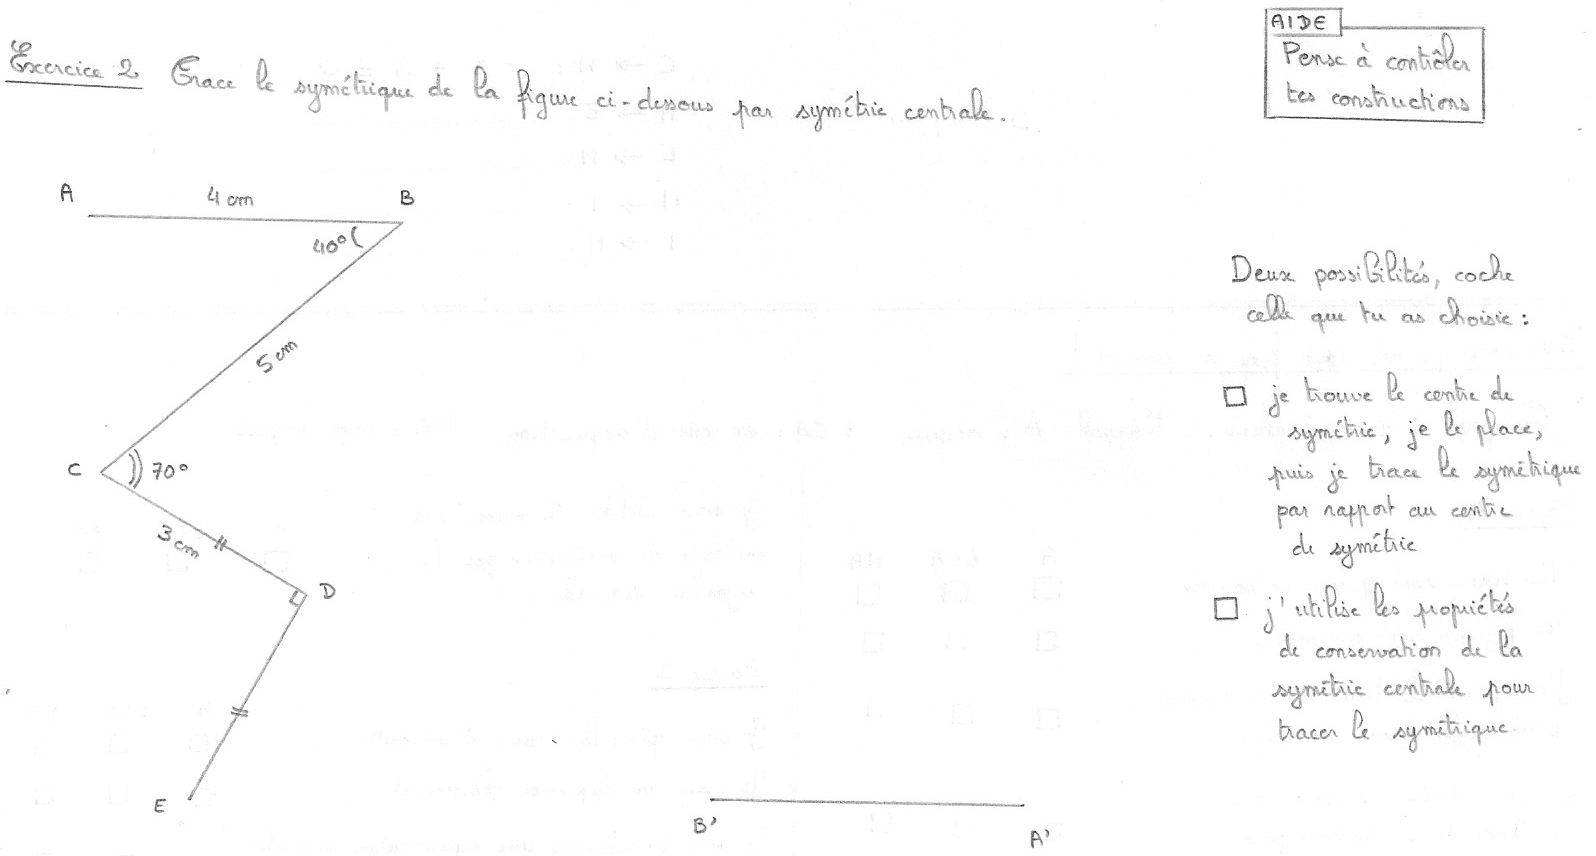
\includegraphics[width=\textwidth]{img/page1-exo2}}
\end{figure}

\subsubsection*{Une faiblesse de l'analyse a priori}
\begin{figure}[!h]
    \center{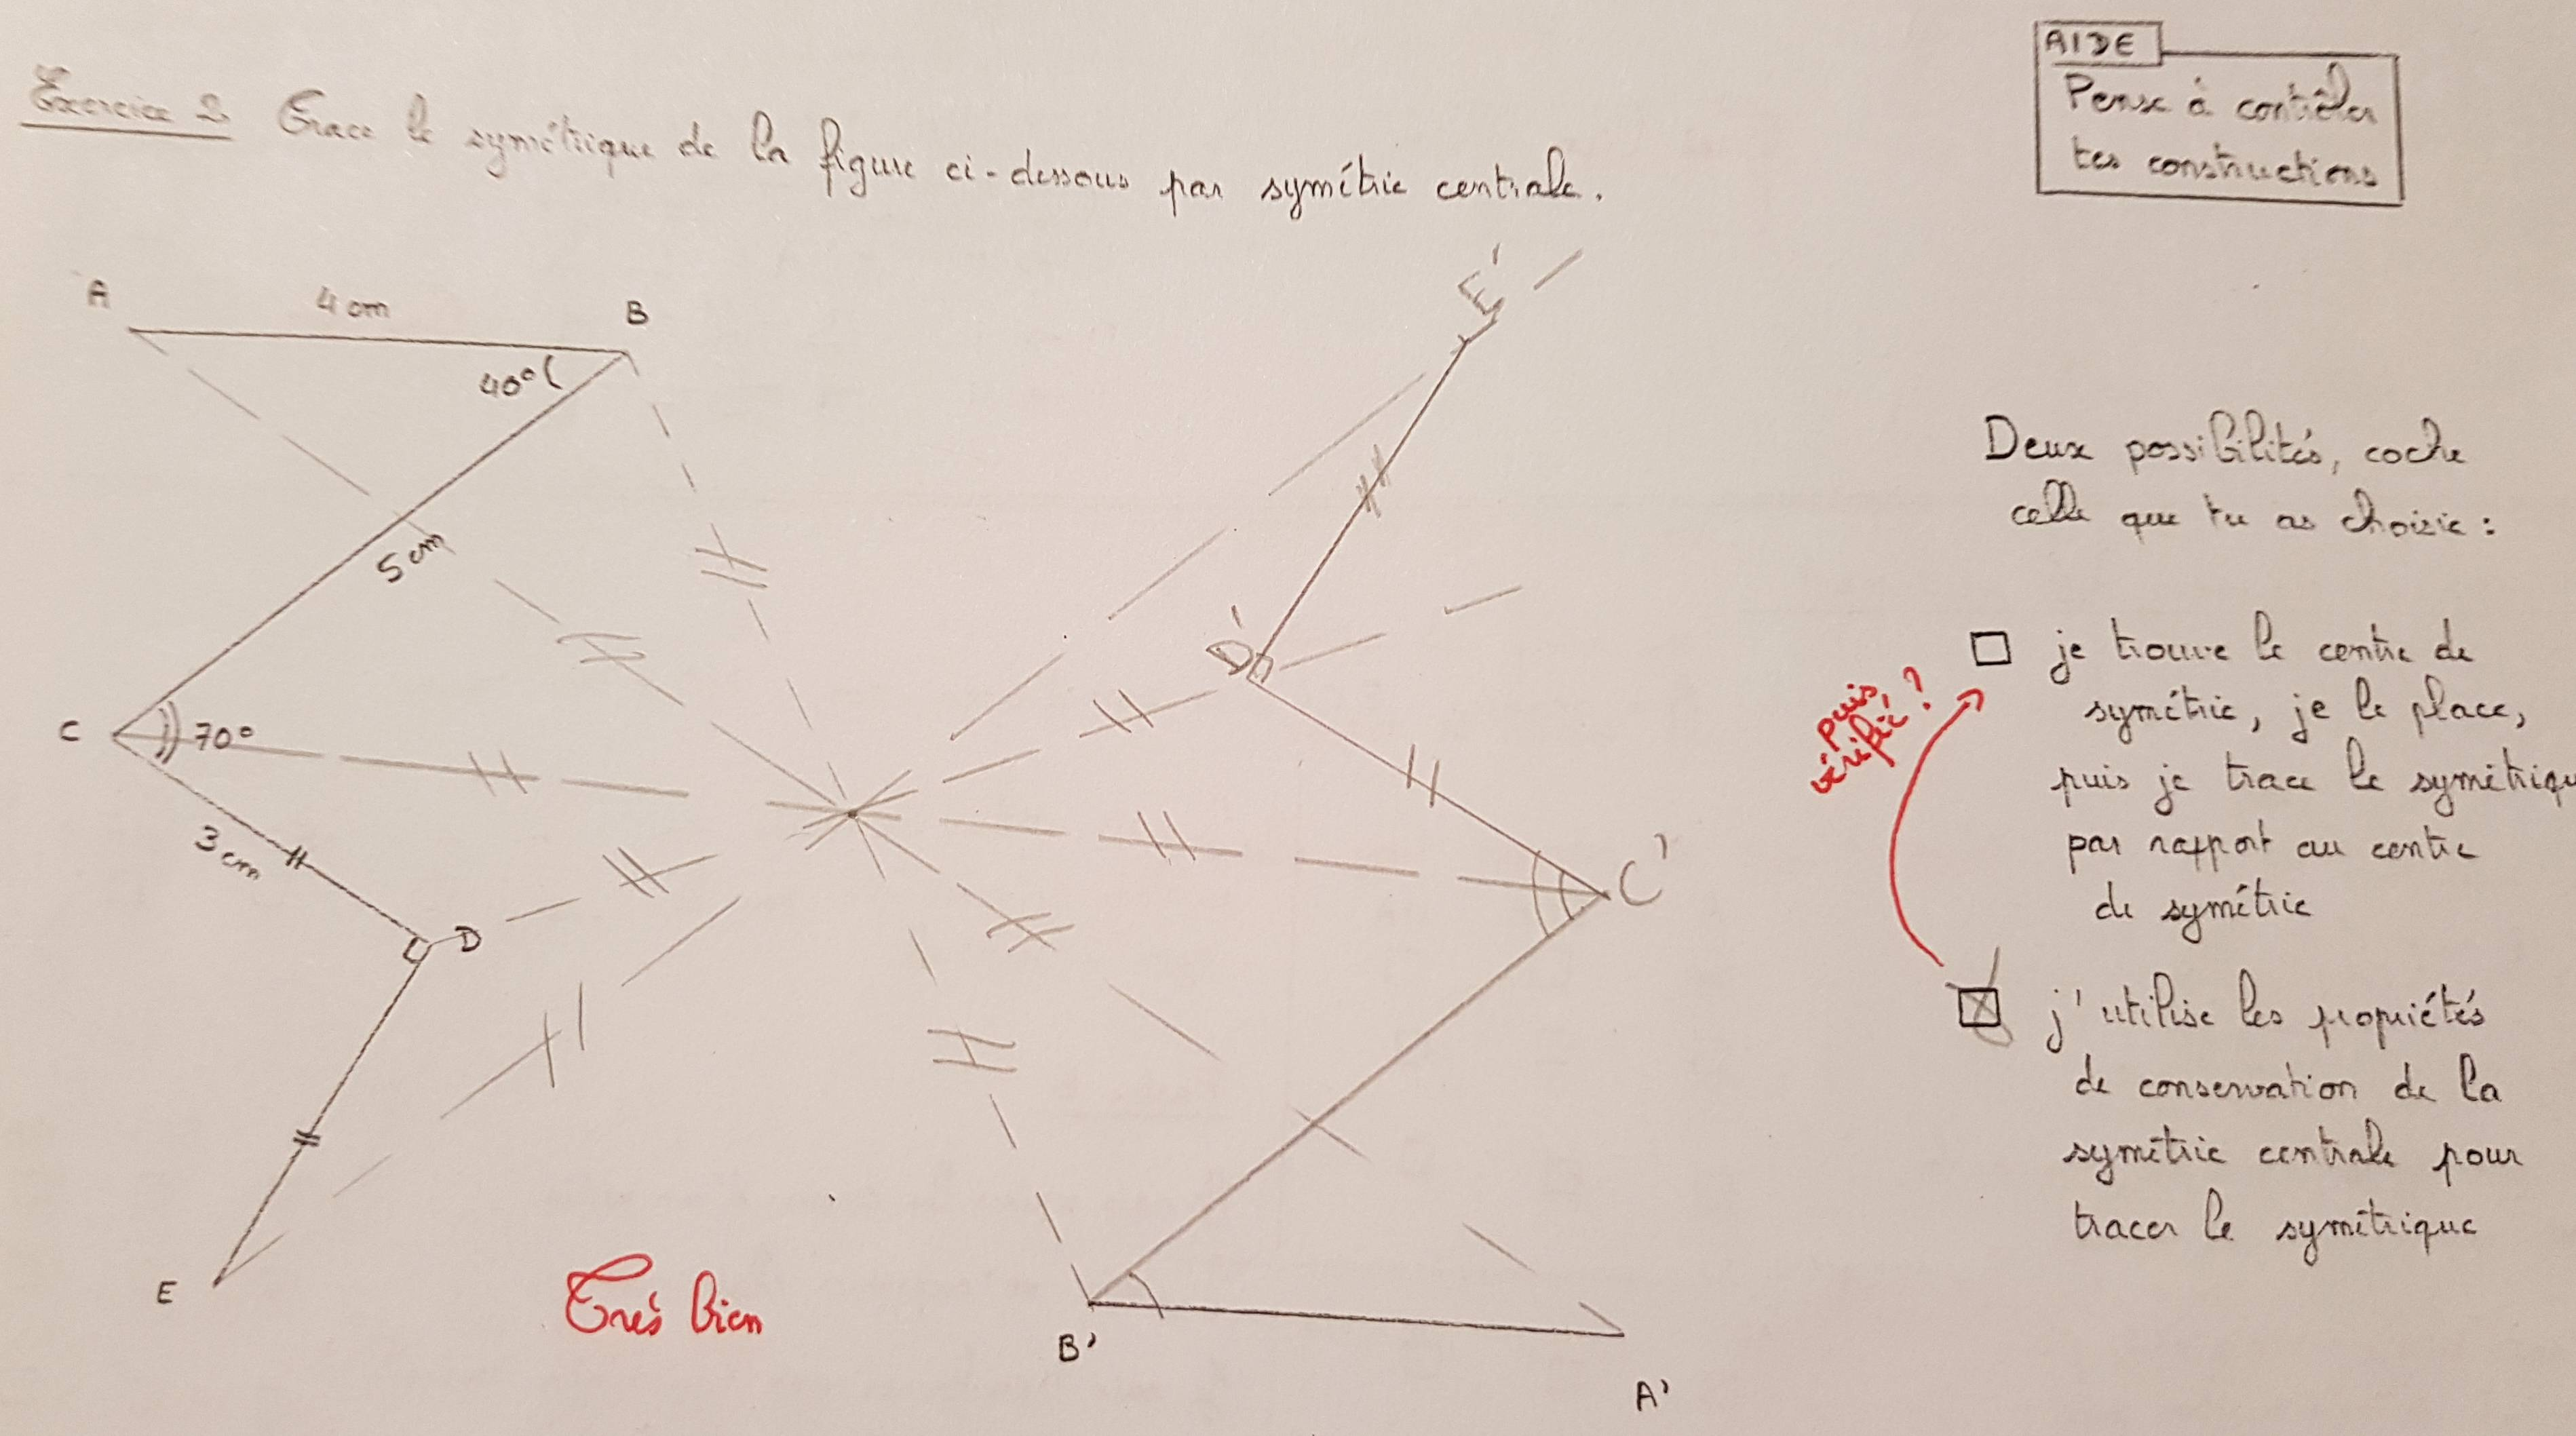
\includegraphics[width=\textwidth]{img/productions/Melyssa.jpg}}
\end{figure}

\clearpage
On constate ici que l'élève a pu suivre deux procédures :
\begin{itemize}
    \item soit elle a utilisé les propriétés de conservation de la symétrie centrale comme elle me l'a indiqué, puis vérifié son travail en déterminant le centre de symétrie et en laissant tous les traits de construction apparents ;
    \item soit elle a utilisé la méthode de construction du centre de symétrie et s'est trompée lorsqu'elle a évalué la stratégie utilisée.
\end{itemize}
En conclusion, l'élève est venue en discuter avec moi en fin d'heure suite à la remarque que j'ai laissée sur sa copie.
Une autre élève m'a indiqué clairement sur sa copie avoir utilisé la seconde stratégie, puis vérifié avec la première stratégie, levant toute ambiguïté, mais cela n'aurait pas dû être nécessaire.\\

On note par ailleurs que je n'a pas corrigé les erreurs de codage (même signe utilisé pour toutes les longueurs).

\subsubsection*{Une erreur courante}\label{confusion}

\begin{figure}[!h]
    \center{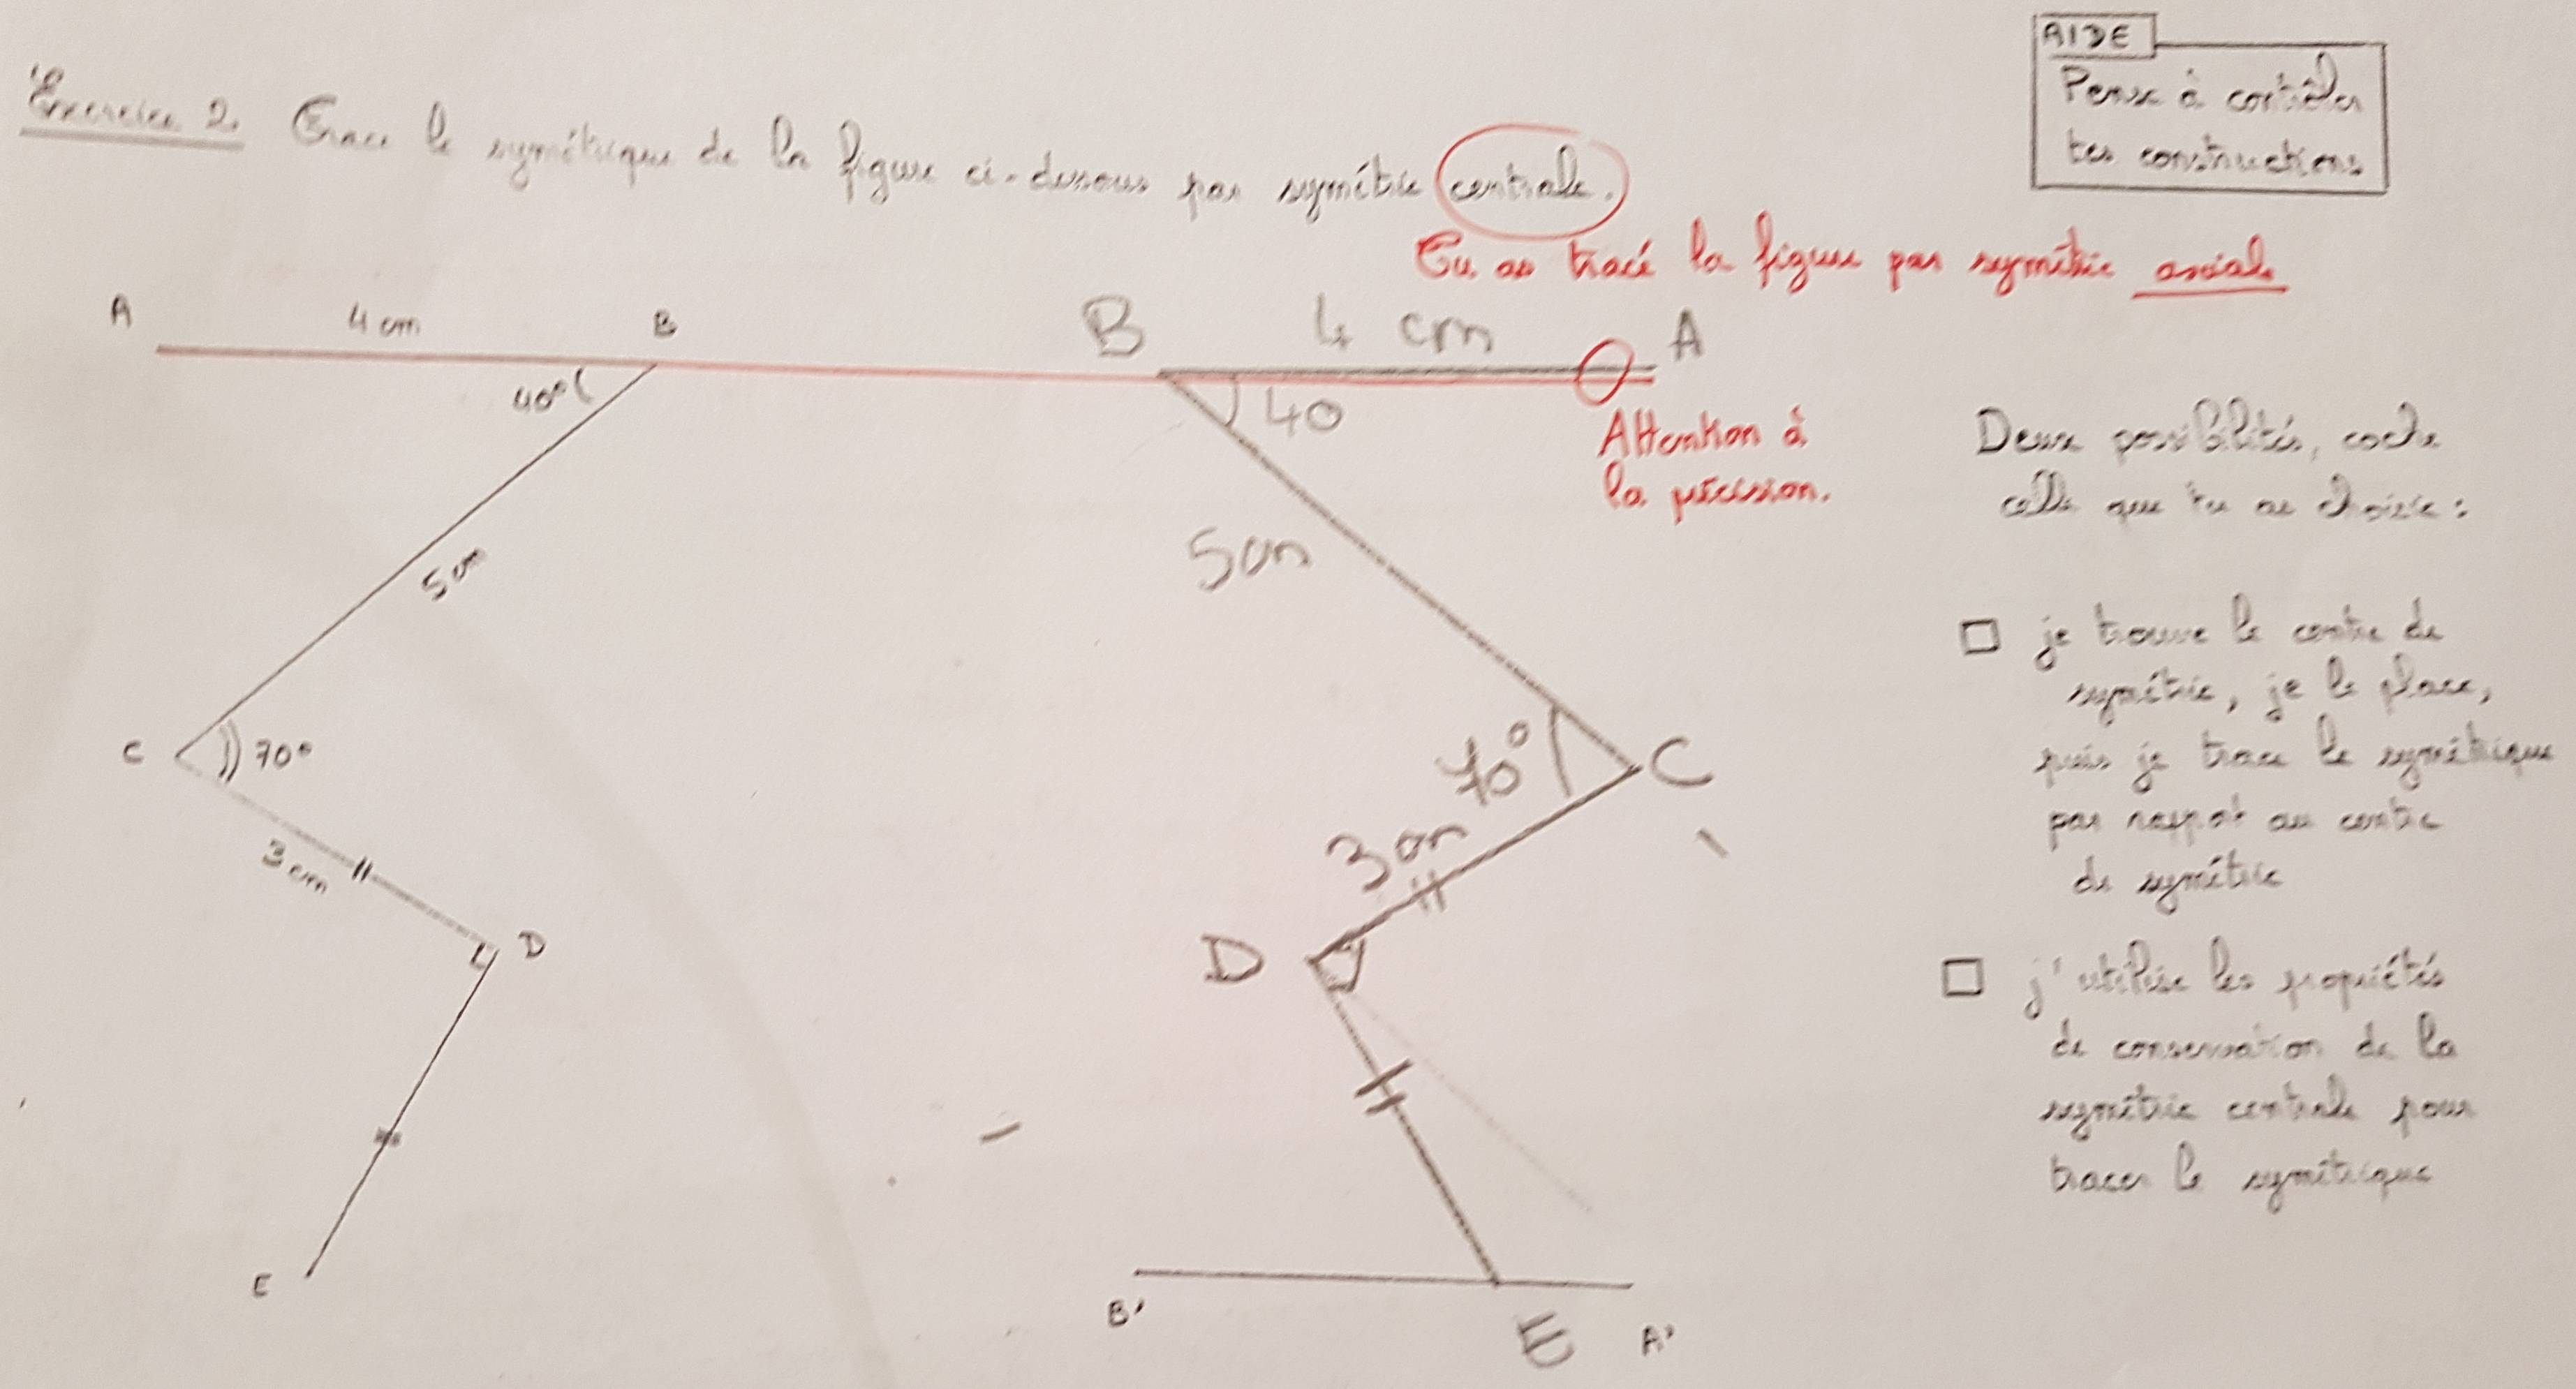
\includegraphics[width=\textwidth]{img/productions/Laeticia.jpg}}
\end{figure}

Cette erreur était attendue. Ici, j'ai noté le manque de précision, c'est un point sur lequel j'avais particulièrement insisté et qui avait été rappelé en début d'évaluation.\\
Cependant, deux copies portant sur la confusion entre symétrie axiale et symétrie centrale ont particulièrement retenu mon attention (voir extrait suivant).

\clearpage
\begin{figure}[!h]
    \center{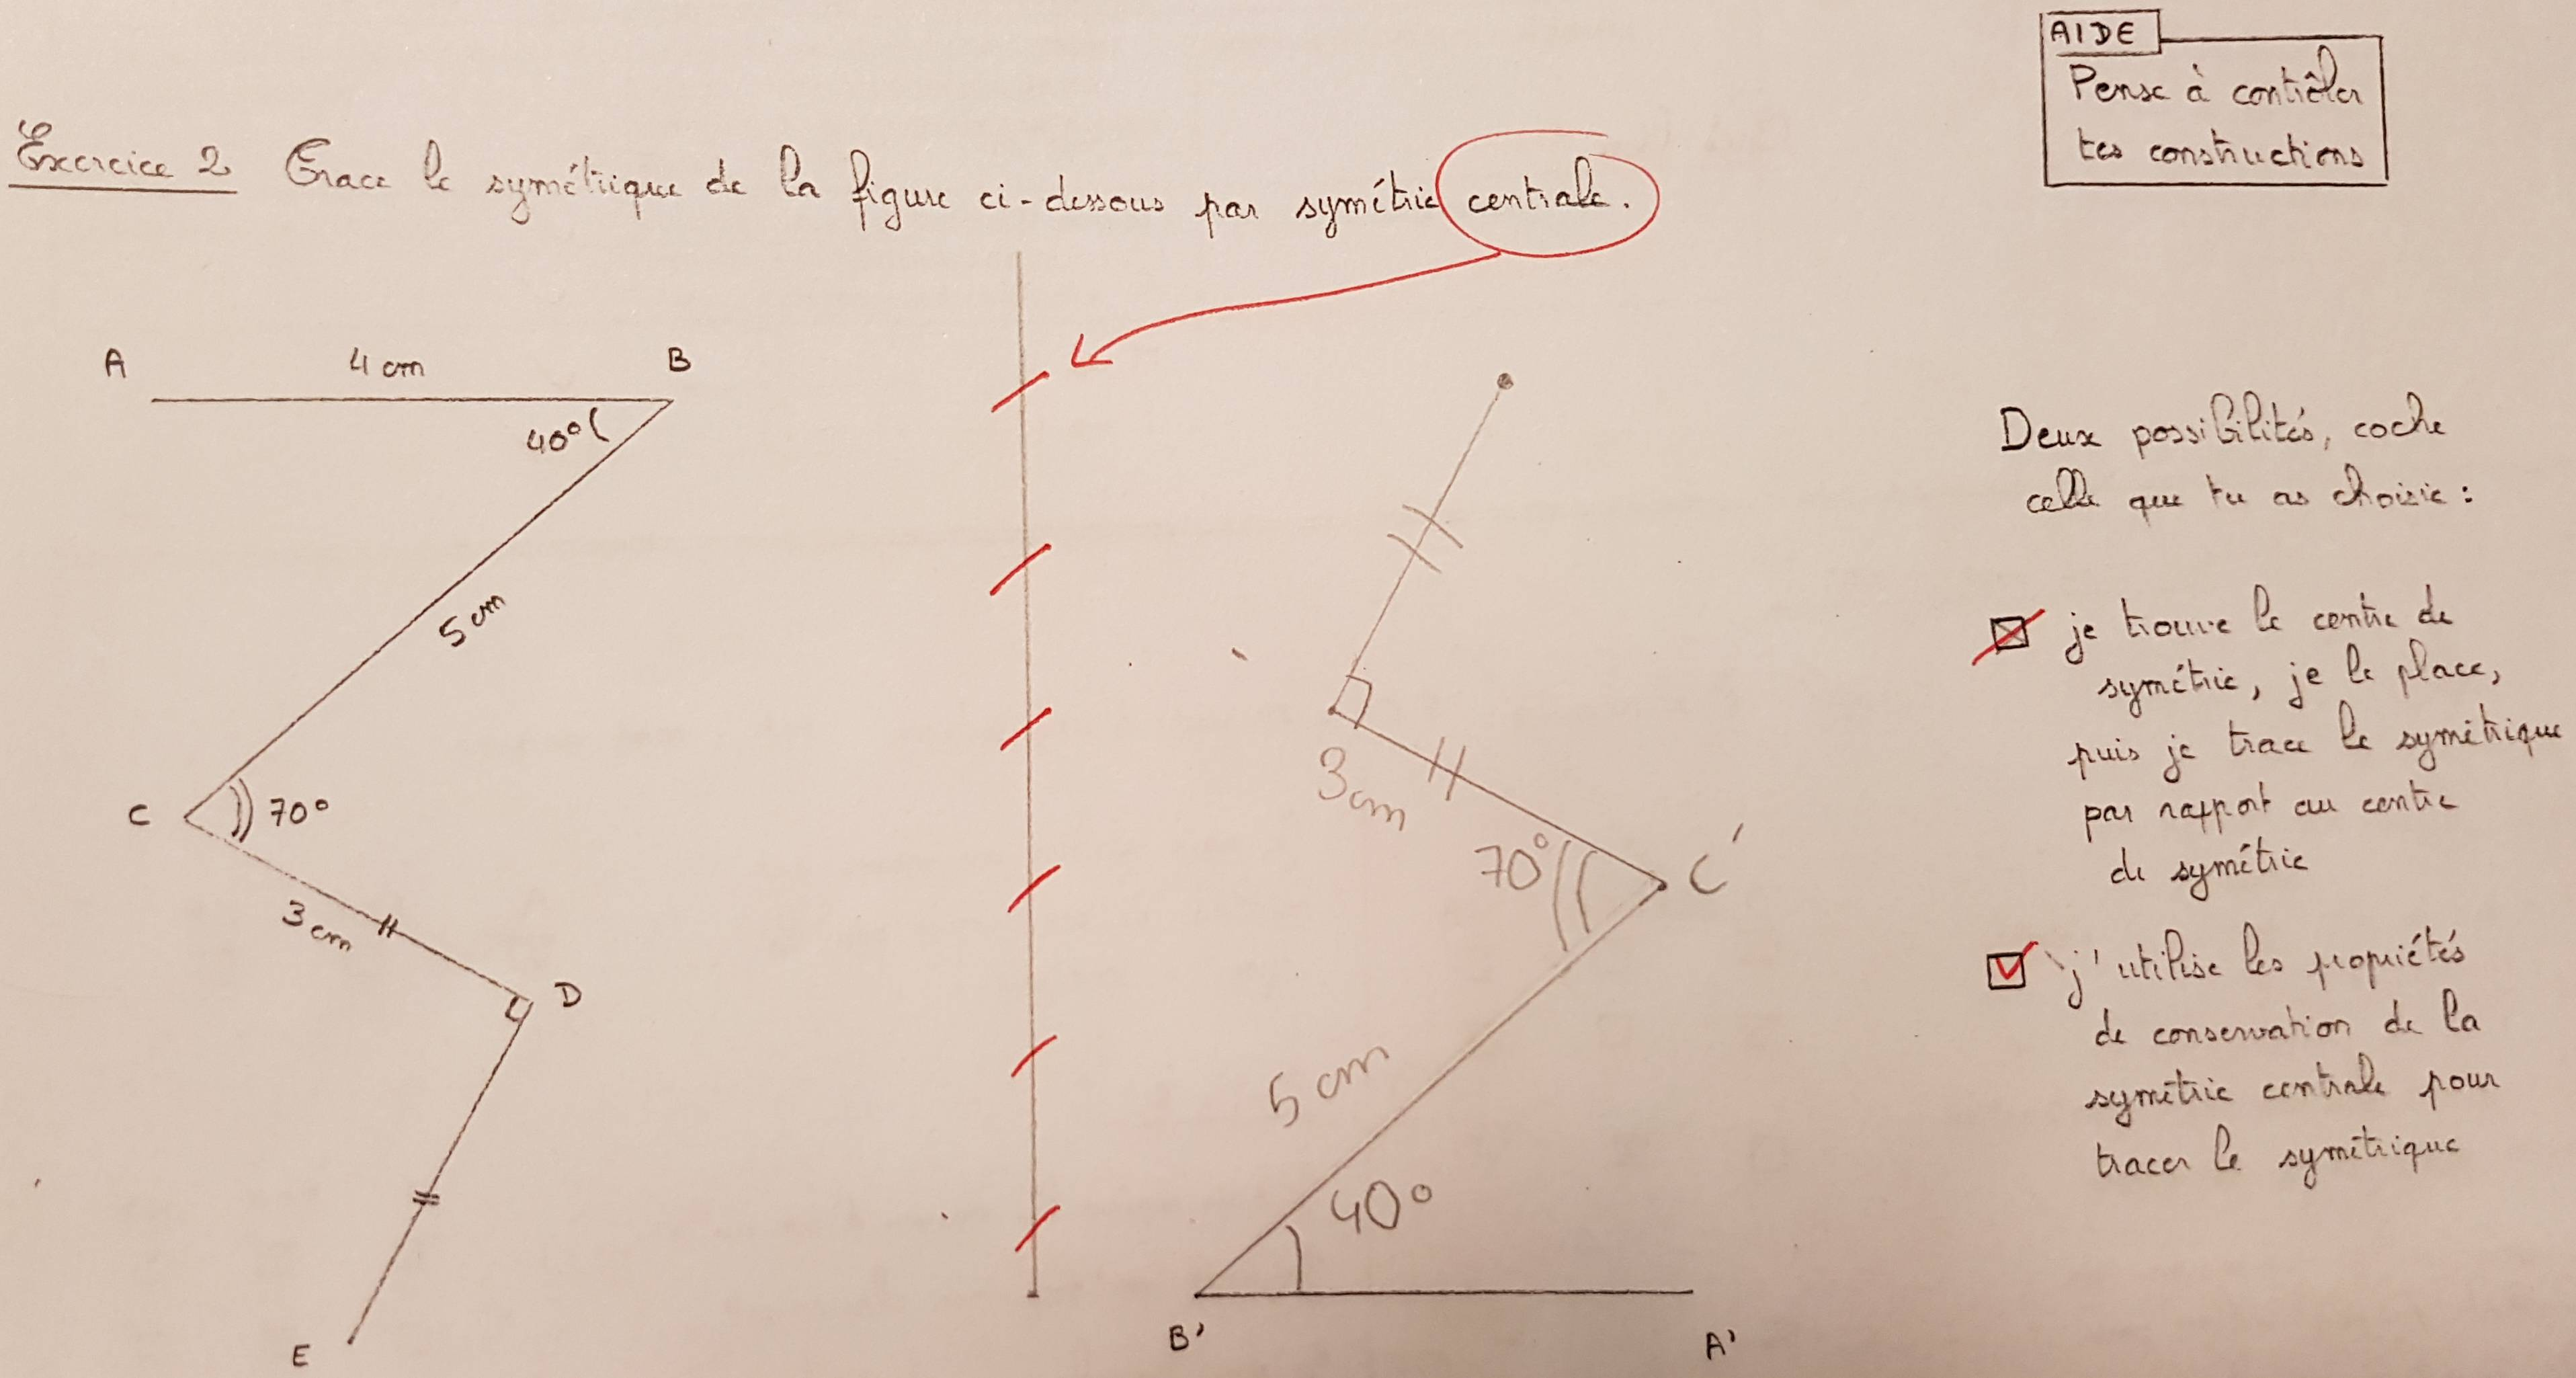
\includegraphics[width=\textwidth]{img/productions/Olivier.jpg}}
\end{figure}

Cette copie est l'une des deux où l'élève a parfaitement répondu à la question, mais où il a tracé un axe vertical pour marquer une symétrie axiale. J'en ai conclu qu'il faudrait lever en aval la possible confusion entre les deux symétries. C'est également grâce à ces deux copies que je me suis rendue compte que l'on n'avait pas assez travaillé la recherche des axes et des centres de symétrie en exercices.

\subsubsection*{Problèmes de temps et de confiance en soi}

L'extrait de copie suivant est l'un des quatre cas où l'élève n'a absolument pas répondu à cet exercice.
\begin{figure}[!h]
    \center{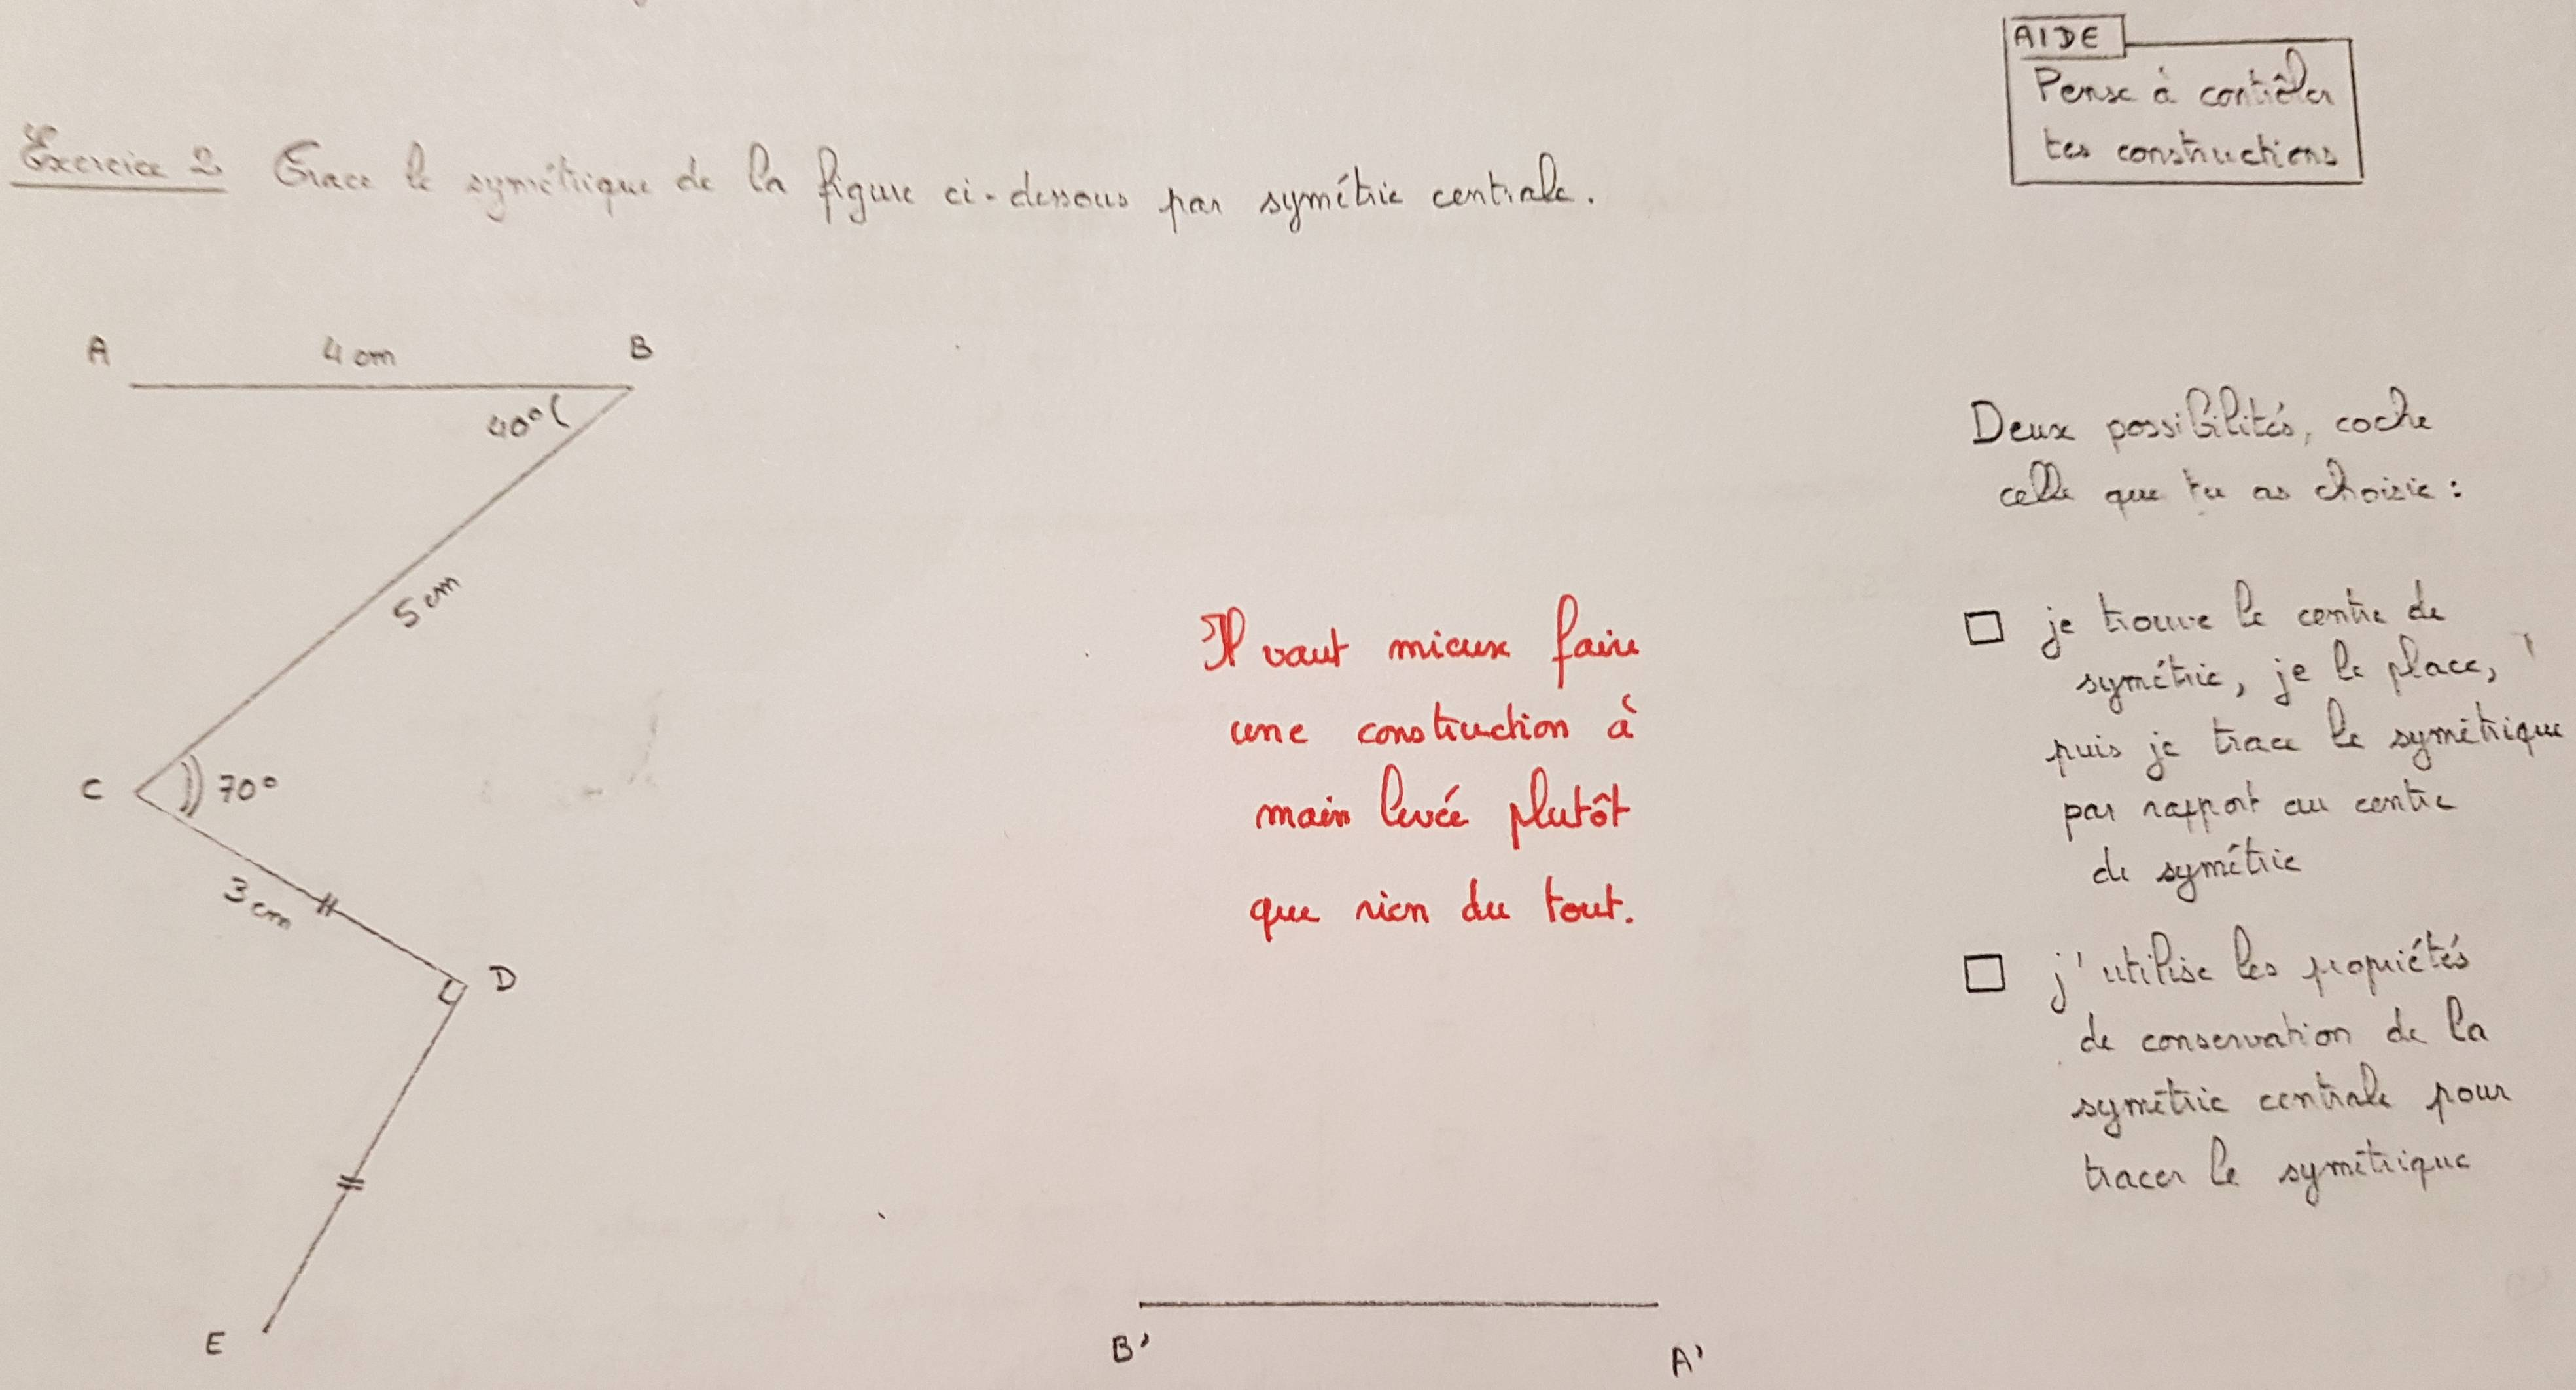
\includegraphics[width=\textwidth]{img/productions/Maissa.jpg}}
\end{figure}

J'ai distingué deux possibilités. La première, l'élève n'a pas osé répondre par manque de confiance en ses capacités. C'était le cas notamment pour un de mes élèves, que j'ai soutenu lors de cette évaluation, sans résultats. 

La deuxième possibilité est que l'élève a manqué de temps. L'élève suivant a choisi de suivre mon conseil lors de l'évaluation et a rendu un travail fait à main levée, qui a été valorisé.

\begin{figure}[!h]
    \center{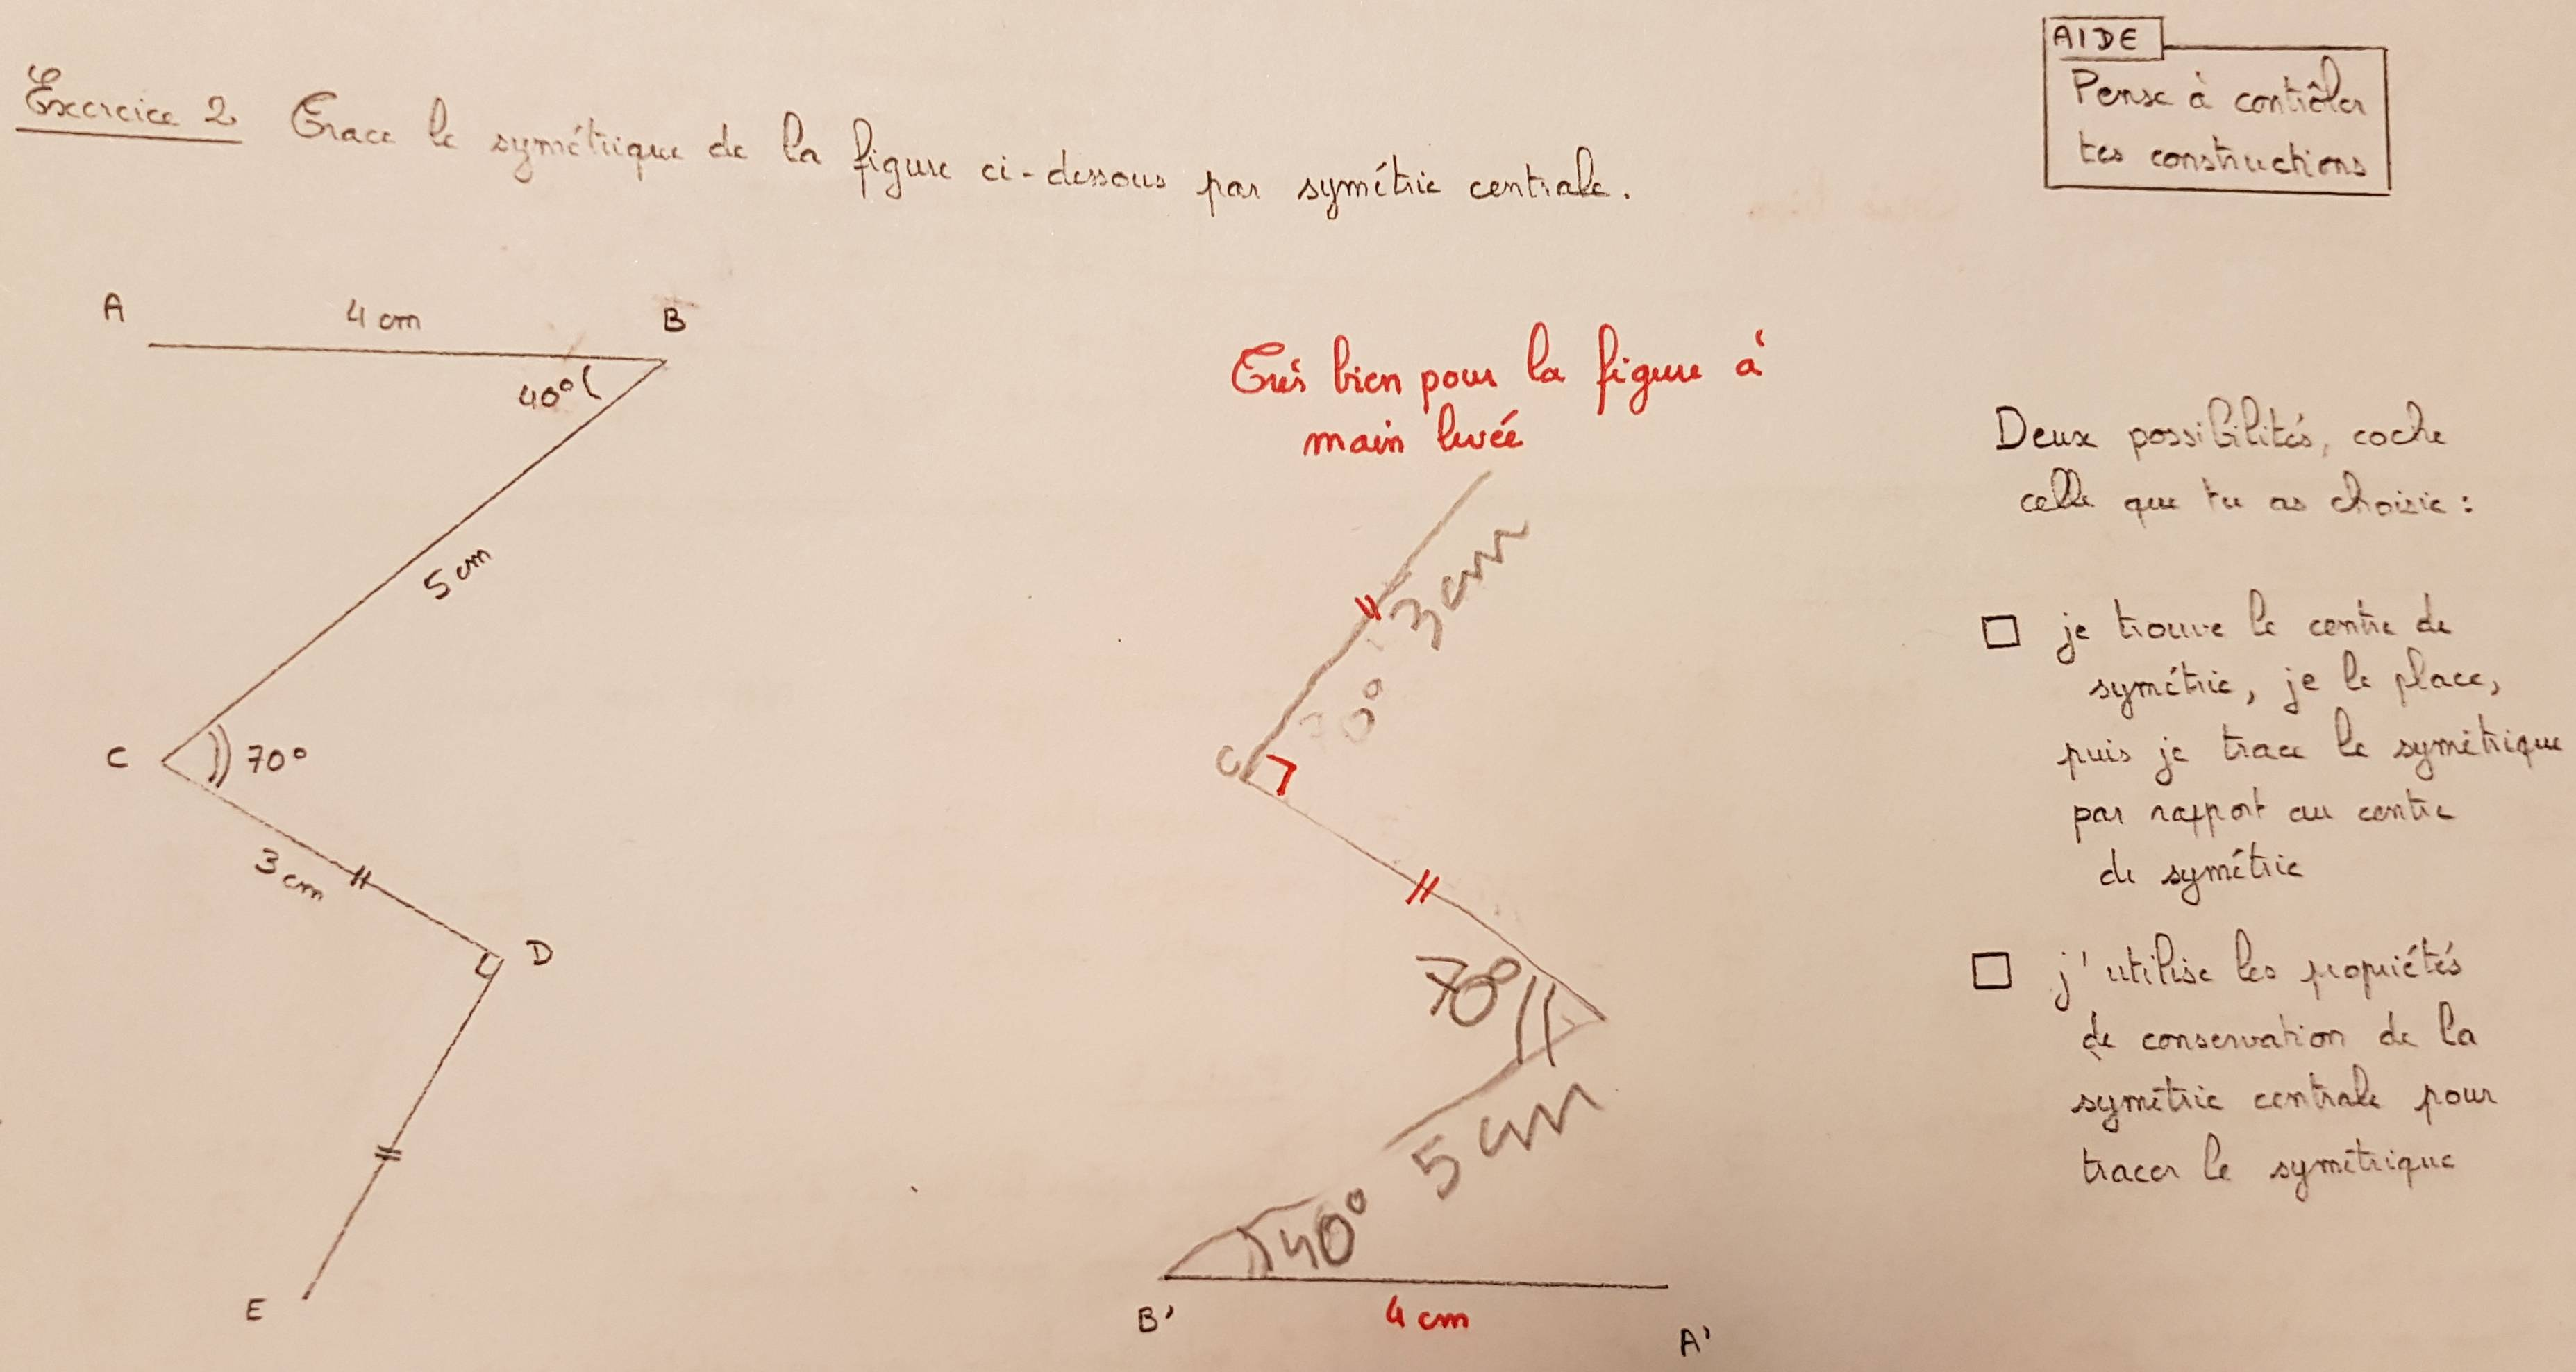
\includegraphics[width=\textwidth]{img/productions/Sidy.jpg}}
\end{figure}

\newpage
\subsection{Travail effectué a posteriori}
%g)le  retour  en  classe  (compte-rendu,  travail  de  remédiation  ou  de  consolidation  des acquis, etc.) et/ou des prolongements possibles
Plusieurs éléments ont été mis en place suite à cette évaluation. Premièrement, c'était la troisième fois que les élèves s'auto-évaluaient et je les ai sondé pour savoir si cela les aidaient. Ils m'ont répondu que la fiche détaillée disponible dans l'annexe \ref{comp} leur était très utile pour mieux comprendre leurs erreurs et orienter leur apprentissage.\\

Lors du rendu de l'évaluation, j'ai beaucoup insisté sur le fait qu'il vaut mieux marquer ou faire quelque chose, plutôt que laisser une question sans réponse. La raison donnée a été que les évaluations ont pour but de les aider à progresser, et que je ne peux les aider à détecter d'éventuelles erreurs de conception que s'ils me laissent une trace de leurs réflexions.\\

J'ai très régulièrement insisté sur les symétries axiales et centrales en questions flash, en particulier sur la recherche d'axes et de centres de symétries suite au constat établi dans la partie \ref{confusion}. J'ai également planifié une activité en salle informatique pour les aider à utiliser Geogebra pour s'entrainer chez eux (voir la précédente analyse de séance). Les élèves peuvent me rendre à tout moment leurs travaux pour une évaluation formative grâce à l'\textit{espace élève} de Pronote. Quelques élèves m'ont déjà soumis leurs constructions. Ils ont également eu une nouvelle évaluation sommative sur cette séquence en janvier.

Concernant la manipulation des nombres relatifs, ils sont travaillés lors de sessions de calcul mental ou lors de séances d'exercices d'applications. La seconde grande évaluation du trimestre~2 contenait deux exercices dédiés aux nombre relatifs avec de nouveaux objectifs.\\

Enfin, j'ai insisté sur la fabrication des fiches de méthodologie. Certains élèves les ont illustrées avec des exemples de construction pas à pas.

% Annexes
\newpage
\subsection{Annexes}

\subsubsection{Fiche d'évaluation jointe aux copies d'élèves}\label{comp}
\begin{figure}[!h]
    \center{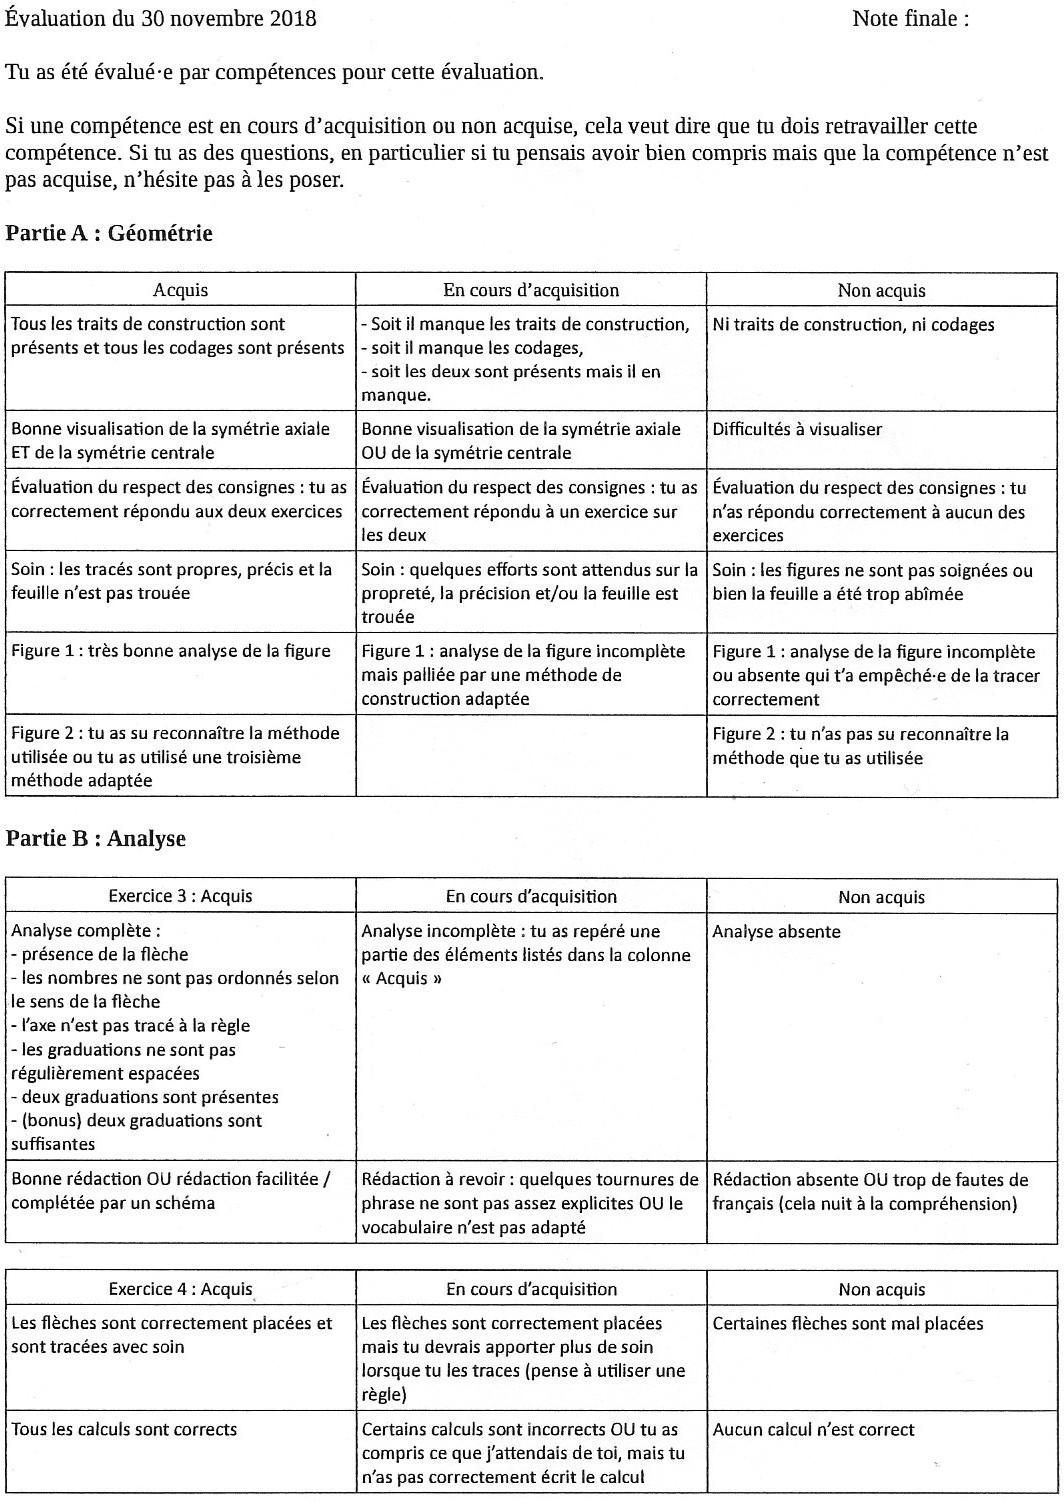
\includegraphics{img/competences}}
\end{figure}

\newpage
\subsubsection{Contenu des fiches méthodologiques}\label{methodo}
\textit{Cette annexe contient le texte brut qui a servi aux élèves pour élaborer leurs fiches.}

\paragraph{Comment faire une construction en géométrie}
Travailler proprement nécessite d'avoir du matériel adapté et de suivre un certain nombre de recommandations :
\begin{itemize}
    \item un crayon HB (ni trop gras, ni trop sec) bien taillé ;
    \item ne pas trop appuyer pour pouvoir gommer ;
    \item anticiper ce que l'on va obtenir (en faisant un petit schéma si besoin) ;
    \item coder la figure au fur et à mesure, conserver les traits de construction ;
    \item vérifier à l'aide de ses connaissances ;
    \item vérifier que le résultat est conforme à l'énoncé.
\end{itemize}

\paragraph{Méthode de construction du symétrique d'une figure par rapport à un centre de symétrie, à la règle uniquement}
\begin{itemize}
    \item choisir le point dont on veut construire le symétrique ;
    \item tracer une demi-droite passant par le point et par le centre de symétrie (à la règle) ;
    \item mesurer la longueur entre le point et le centre de symétrie (à la règle) ;
    \item reporter cette longueur de l'autre coté du centre de symétrie et marquer le point ;
    \item \textit{coder la figure} ;
    \item recommencer pour tous les autres points de la figure.
\end{itemize}

\paragraph{Méthode de construction du symétrique d'une figure par rapport à un centre de symétrie, à la règle et au compas}
\begin{itemize}
    \item choisir le point dont on veut construire le symétrique ;
    \item tracer une demi-droite passant par le point et par le centre de symétrie (à la règle) ;
    \item mesurer la longueur entre le point et le centre de symétrie (au compas) ;
    \item reporter cette longueur de l'autre coté du centre de symétrie (au compas) et marquer le point\\
    \textit{(on peut faire ces deux étapes en une seule en plaçant la pointe du compas sur le centre de symétrie et en traçant le cercle passant par le point)} ;
    \item \textit{coder la figure} ;
    \item recommencer pour tous les autres points de la figure.
\end{itemize}

\newpage
\subsubsection{Devoir maison du papillon}\label{papillon}
\textit{Cette annexe contient l'image qui a servi aux élèves pour travailler la construction de figures en géométrie. La symétrie centrale leur permettait de compléter le motif des ailes et la symétrie axiale leur permettait de faire l'aile gauche du papillon.}

\textit{Le petit papillon complet en haut à gauche de l'image leur a été distribué sur une feuille séparée pour leur servir de guide.}
\begin{figure}[!h]
    \center{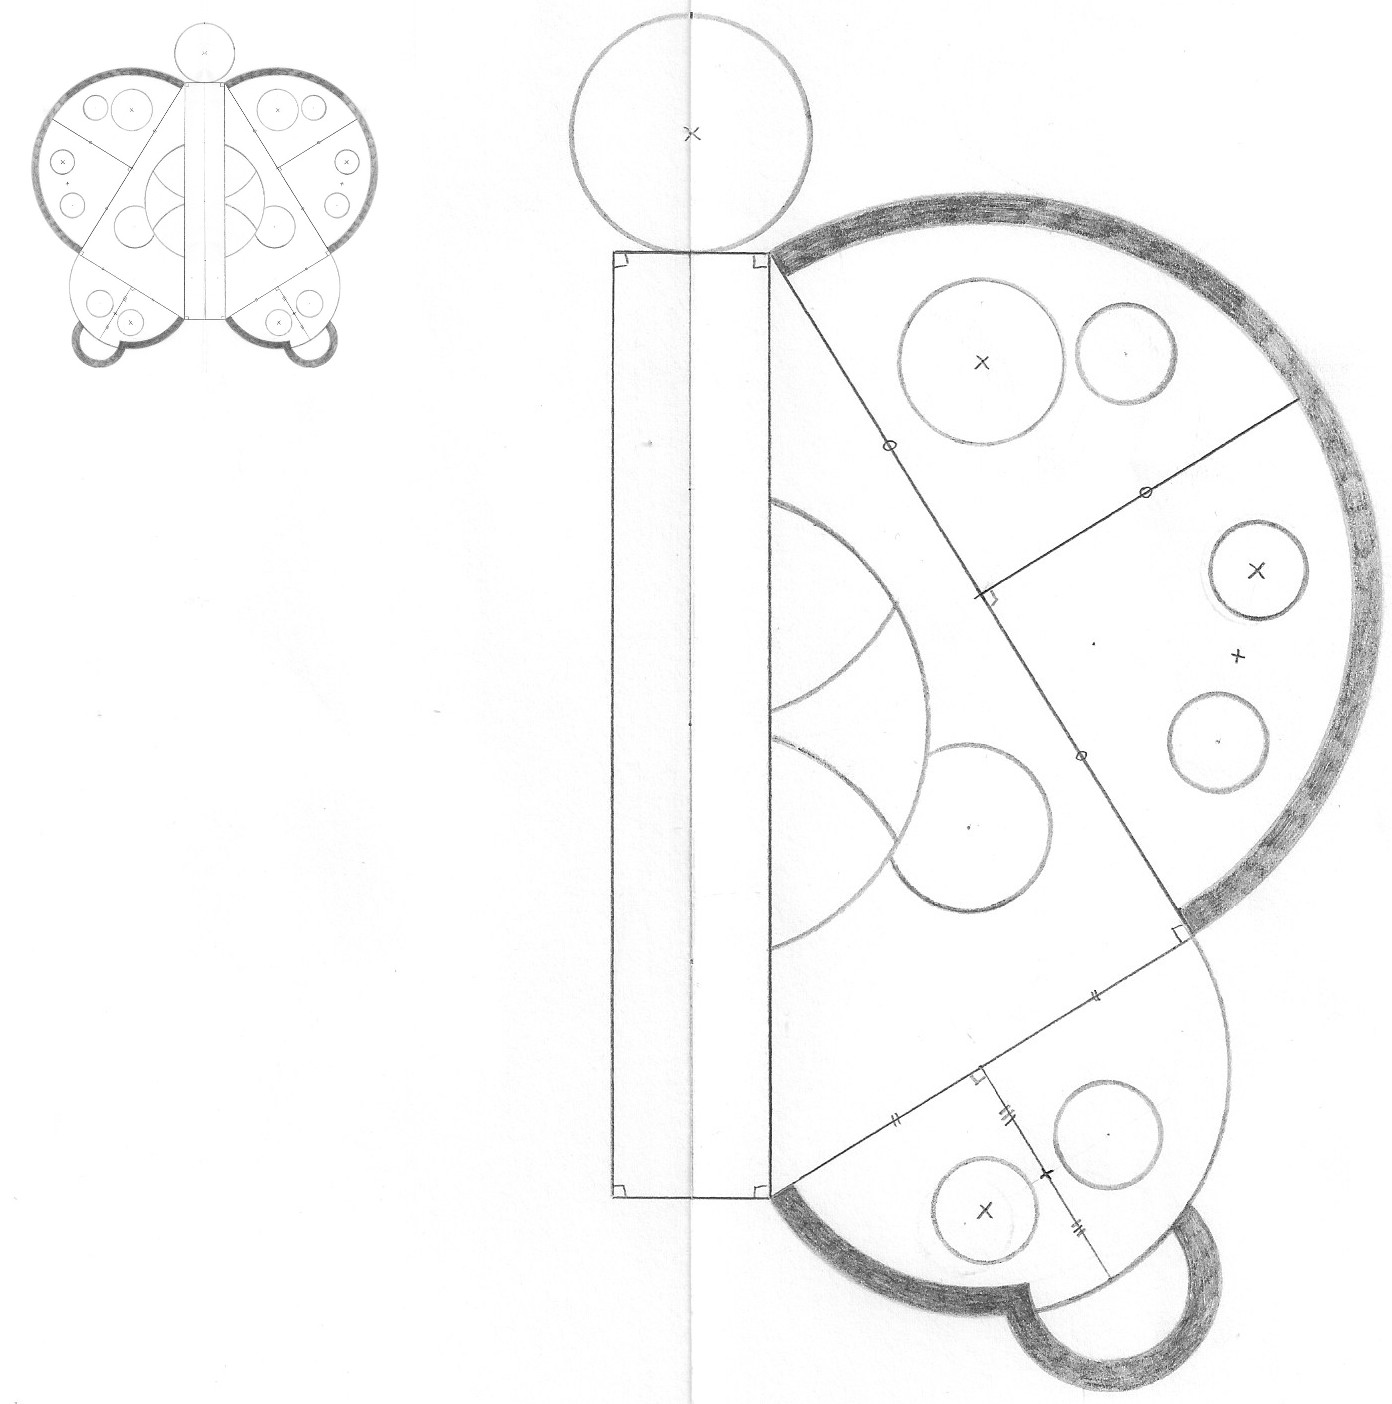
\includegraphics{img/papillon2}}
\end{figure}